% Full title as you would like it to appear on the page
\chapter{Training a Convolutional Neural Network To Predict The Local Wavefront}
\label{chap:cnn}
\chaptermark{Training a CNN}

\epigraph{Uncrumpling paper balls is what machine learning is about: finding neat representations for complex, highly folded data manifolds.}{Fran\c{c}ois Chollet}

In the first step, we use a convolutional neural network (CNN) to predict the relationship between donuts and their corresponding local wavefronts. There are three inputs to the network: the $256\ \times\ 256$ pixel donut image $D$, the position $r$ of the sensor. This position $r = (x,y,d)$ is comprised of the $(x,y)$ field position in radians, and the offset $d$ along the z-axis indicating whether the defocus is intra-focal or extra-focal. The output is the vector of Zernike coefficients $\alpha \in \mathbb{R}^{18}$. The sub-problem is to find a function approximator $\phi$,

\begin{equation*}
\phi(D, r) \to \alpha(x,y) \text{ such that } W(u,v|x,y) \approx \sum_{j=4}^{21}\alpha_j(x,y)Z_j(u,v)
\end{equation*}

Predicting the local wavefront $W(u,v|x,y)$ from donuts and their metadata is an intrinsically challenging problem because the optics contribution to the image is sometimes degenerate with, and typically subdominant to, the atmospheric contribution. Thus, even for very bright donuts with no effective sources of background noise, the model will have a systematic ceiling. In this section, we demonstrate that a CNN can produce accurate estimates despite this challenge.

\section{Network Architecture}

\begin{figure}[!htbp]
\begin{center}
\begin{tabular}{c}
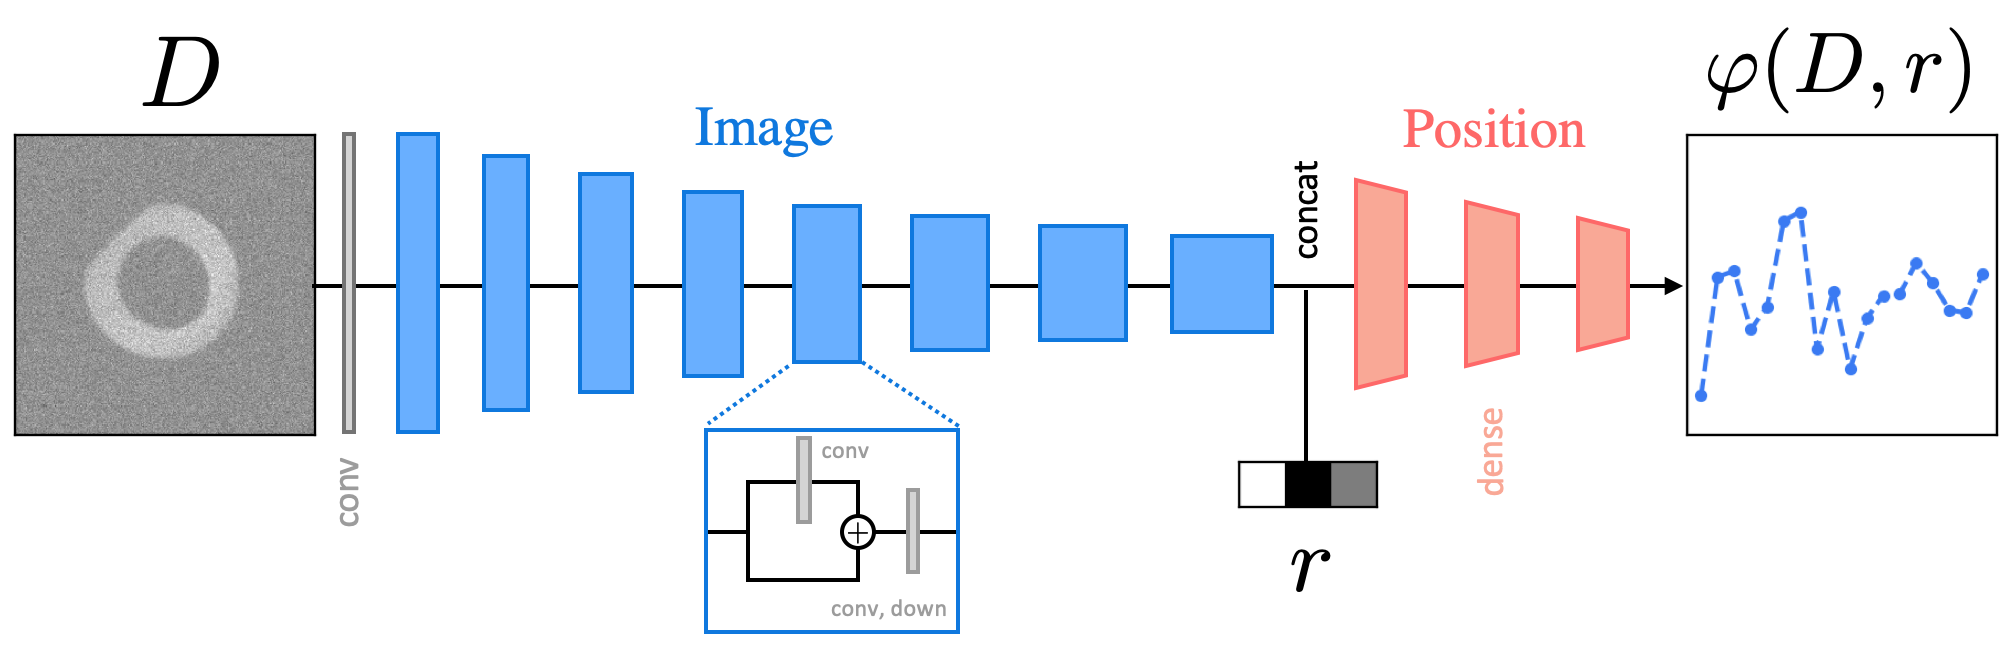
\includegraphics[width=\textwidth]{figs/cnn/arch.png}
\end{tabular}
\end{center}
\caption[Network Architecture]{The network architecture and example inputs and output. The image network is in blue and the position network is in red.\label{fig:arch}}
\end{figure}


Modern CNN architectures are governed by an astounding number of design decisions and hyper-parameter options. Here we show that a simple network can make highly accurate wavefront estimates without many additional design or hyper-parameter optimizations. This shows that this step can also serve as a network in other optics algorithms.

The network, shown in Figure \ref{fig:arch}, has two sub-networks: an image network and a position network. e will describe the architecture through the convolutions that are applied and how they change the data tensors. Each 2-dimensional convolution or linear layer, except the final linear layer, is followed by a 2-dimensional batch normalization layer (batchnorm) and a rectified linear activation (ReLU) \cite{726791, batchnorm, relu}. The batch normalization protects against covariate-shift and provides weak regularization and the ReLU activation introduces non-linearity. 

The image network reduces the donut image to a 1024 dimensional vector. The first component is a convolution that increases the depth of the input from 1 to 8, and retains the 256 by 256 height and width. This is followed by a sequence of 8 Down-Blocks. Each Down-Block has an initial convolution that does not change the tensor dimensions, followed by a convolution that increases the depth by a factor of 2 and reduces the height and width by a factor of 2. There is a skip connection between these two convolutions for better gradient flow \cite{resnet}. In the 8th and final Down-Block, the depth is not increased. Thus by the end of these steps we have a depth of $\text{depth} = 8 \cdot 2^7 = 1024$ and $\text{height} = \text{width} = 256 \cdot 2^{-8} = 1$. This $1 \times 1 \times 1024$ output is a learned representation of the input image. In total, the image network has 28,326,360 trainable parameters.

The position network combines the $1 \times 1 \times 1024$ output from the image network vector with the 3-dimensional position input $r=(x,y,d)$ and estimates the 18 local wavefront coefficients. It first concatenates and flattens these tensors into a combined 1027-dimensional tensor. Then three linear layers reduce the dimensionality to 266, 69, and 18 respectively (the sequential dimensions are log-linear). After the first linear layer we insert a dropout layer with a 90\% keep probability \cite{10.5555/2999134.2999257} to improve generalization. In total, the position network has 293,801 trainable parameters. 

We developed the model in PyTorch \cite{pytorch}. We determined this balance of parameters between sub-networks through testing. In the next Section we describe how the network is trained. 

\section{Training, Validation, and Testing}

\begin{figure}[!htbp]
\begin{center}
\begin{tabular}{c}
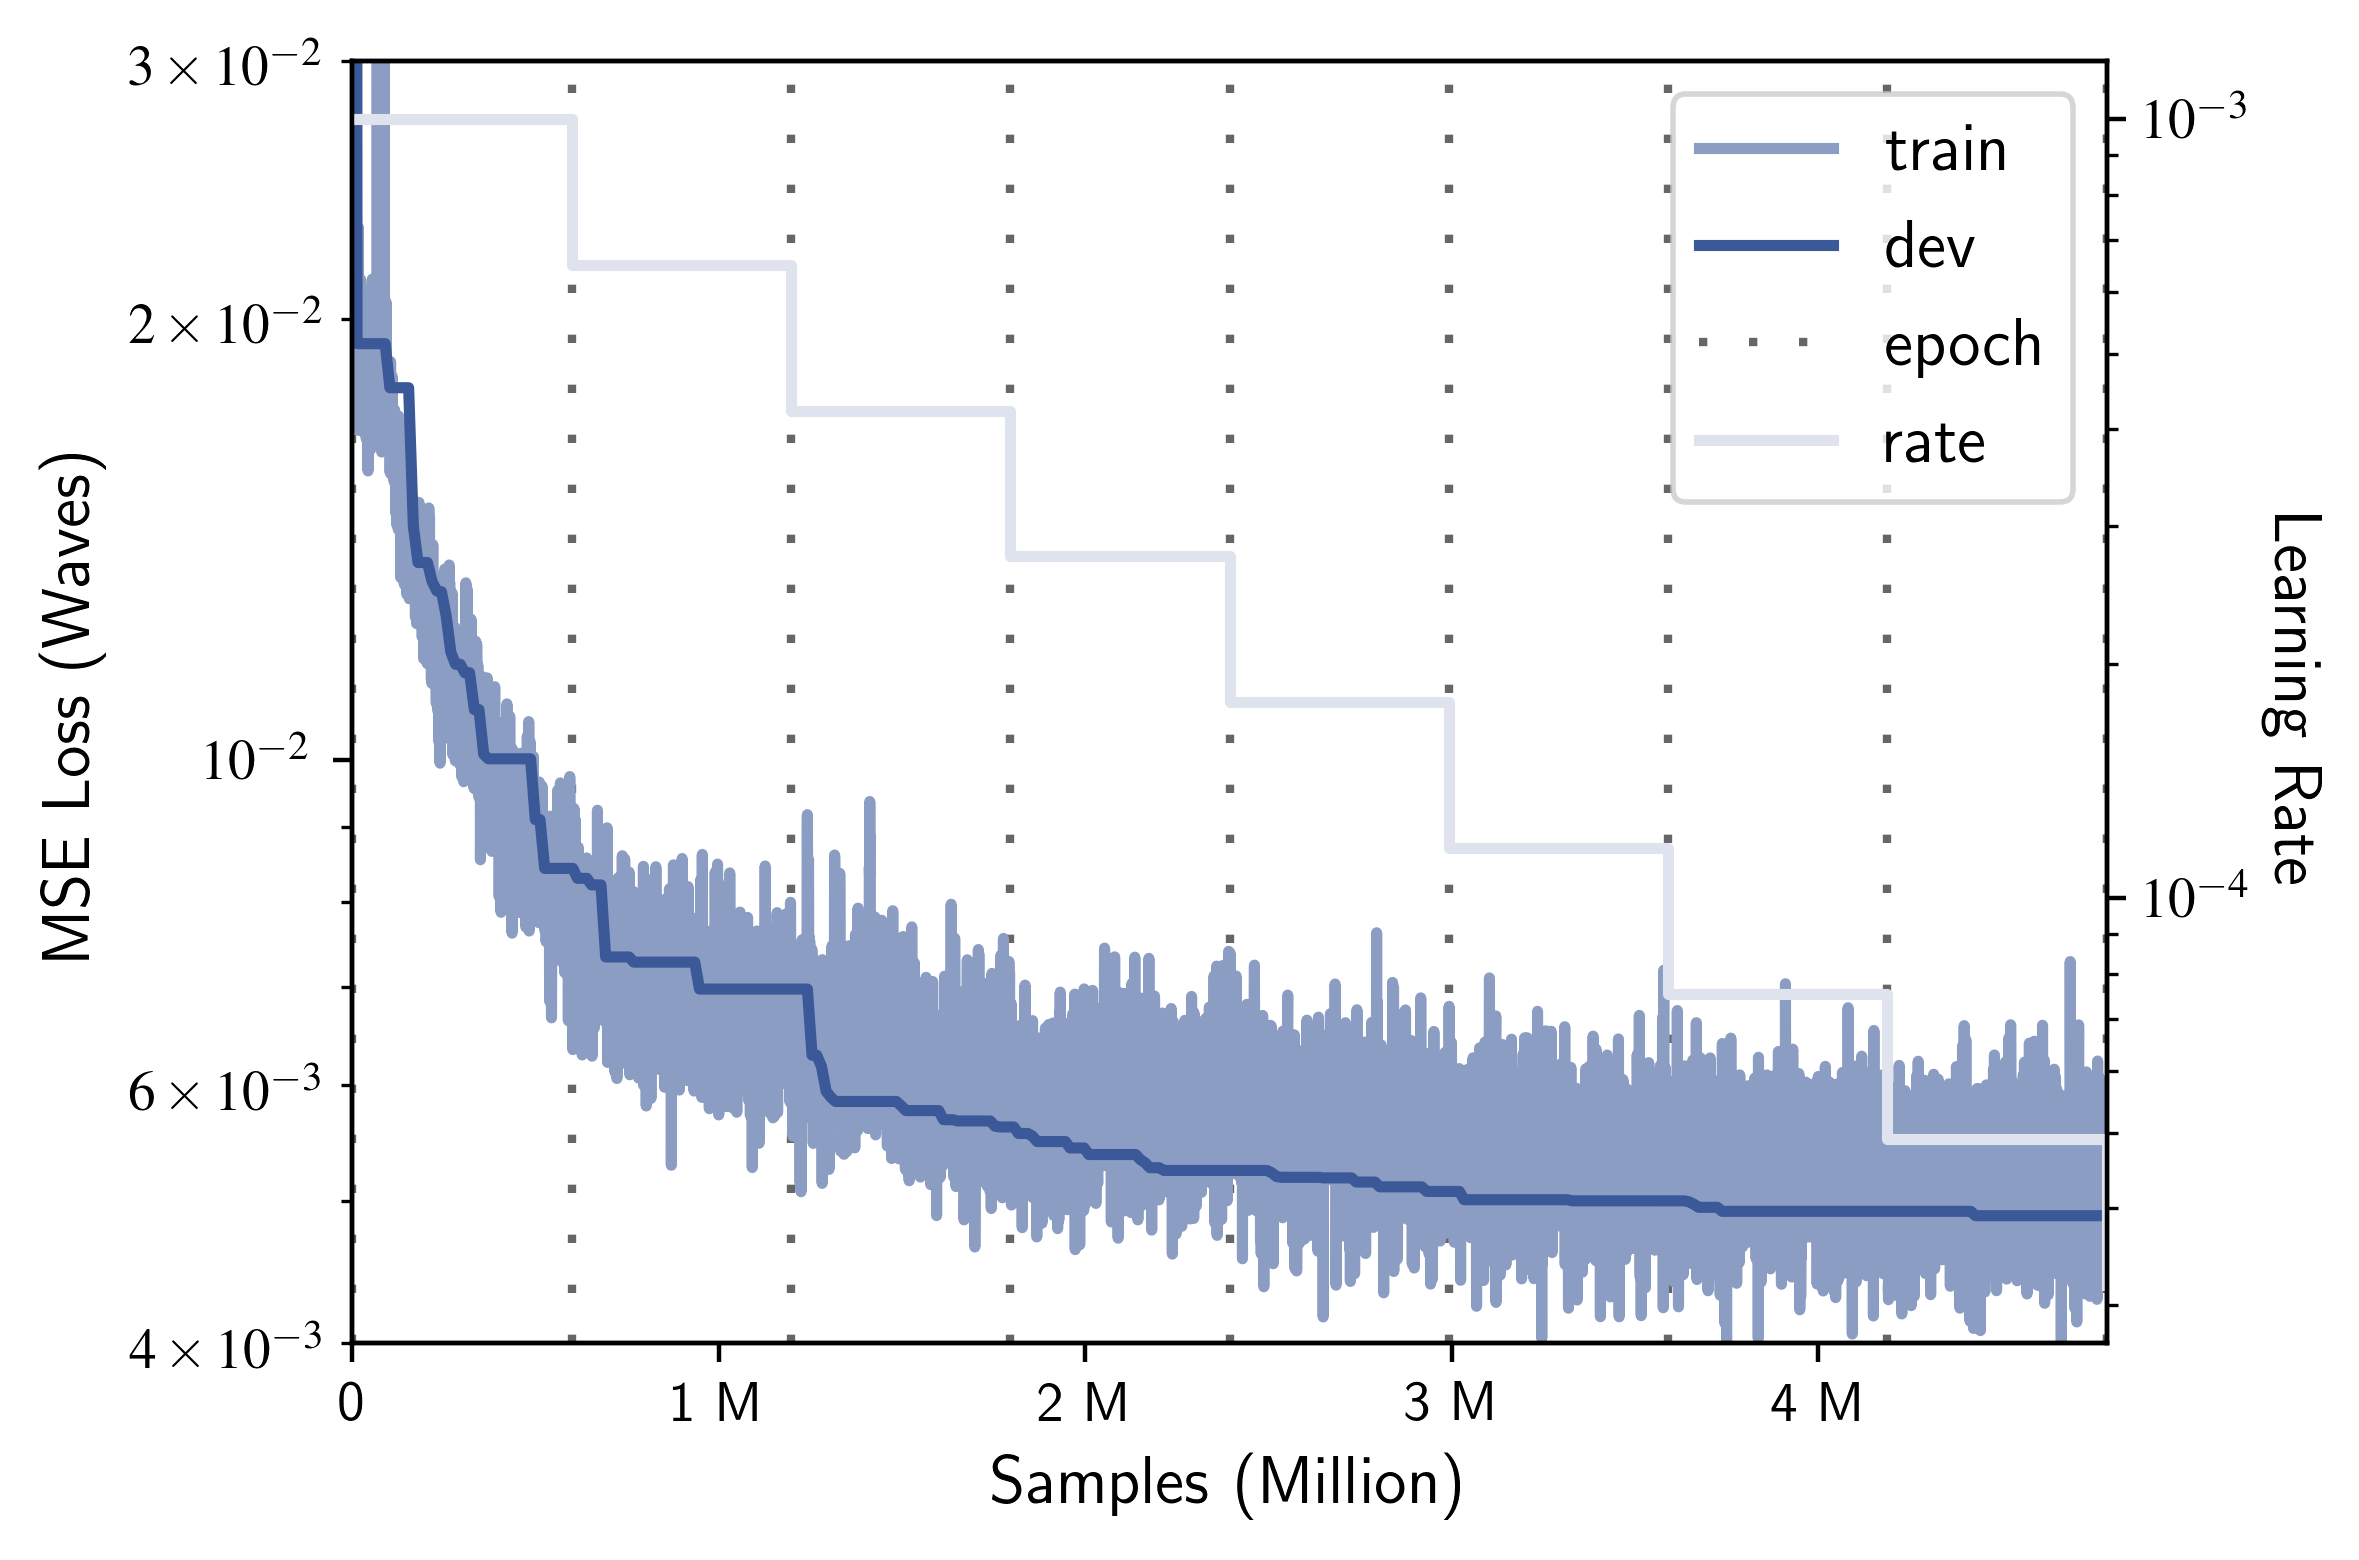
\includegraphics[width=\textwidth]{figs/cnn/training_curve.png}
\end{tabular}
\end{center}
\caption[Training Curve]{The training loss (train), validation loss (dev), and learning rate versus the number of samples used for training the neural network. The MSE loss corresponds to the y-axis on the left; the learning rate corresponds to the y-axis on the right.\label{fig:train}}
\end{figure}

In addition to the large number of decisions that go into the network architecture, there are also a lot of decisions on the configuration of the training. For the loss function, we use the mean-squared-error (MSE) between the estimated and true wavefront coefficients and found it to be superior to the mean-absolute-error. We evaluate batches of 64 samples at a time and use the Adam optimizer to compute the parameter updates for the backward pass after computing the loss function in the forward pass \cite{adam}. We train the model for 8 epochs over the donut dataset. After each epoch we multiply the learning rate by a factor of 0.65. Every 200 batches, we evaluate the MSE of the model on the donut validation set, and keep the best model. Figure \ref{fig:train} shows the training and validation (dev) errors, and the learning rate, versus the number of training samples.

\begin{figure}[!htbp]
\begin{center}
\begin{tabular}{c}
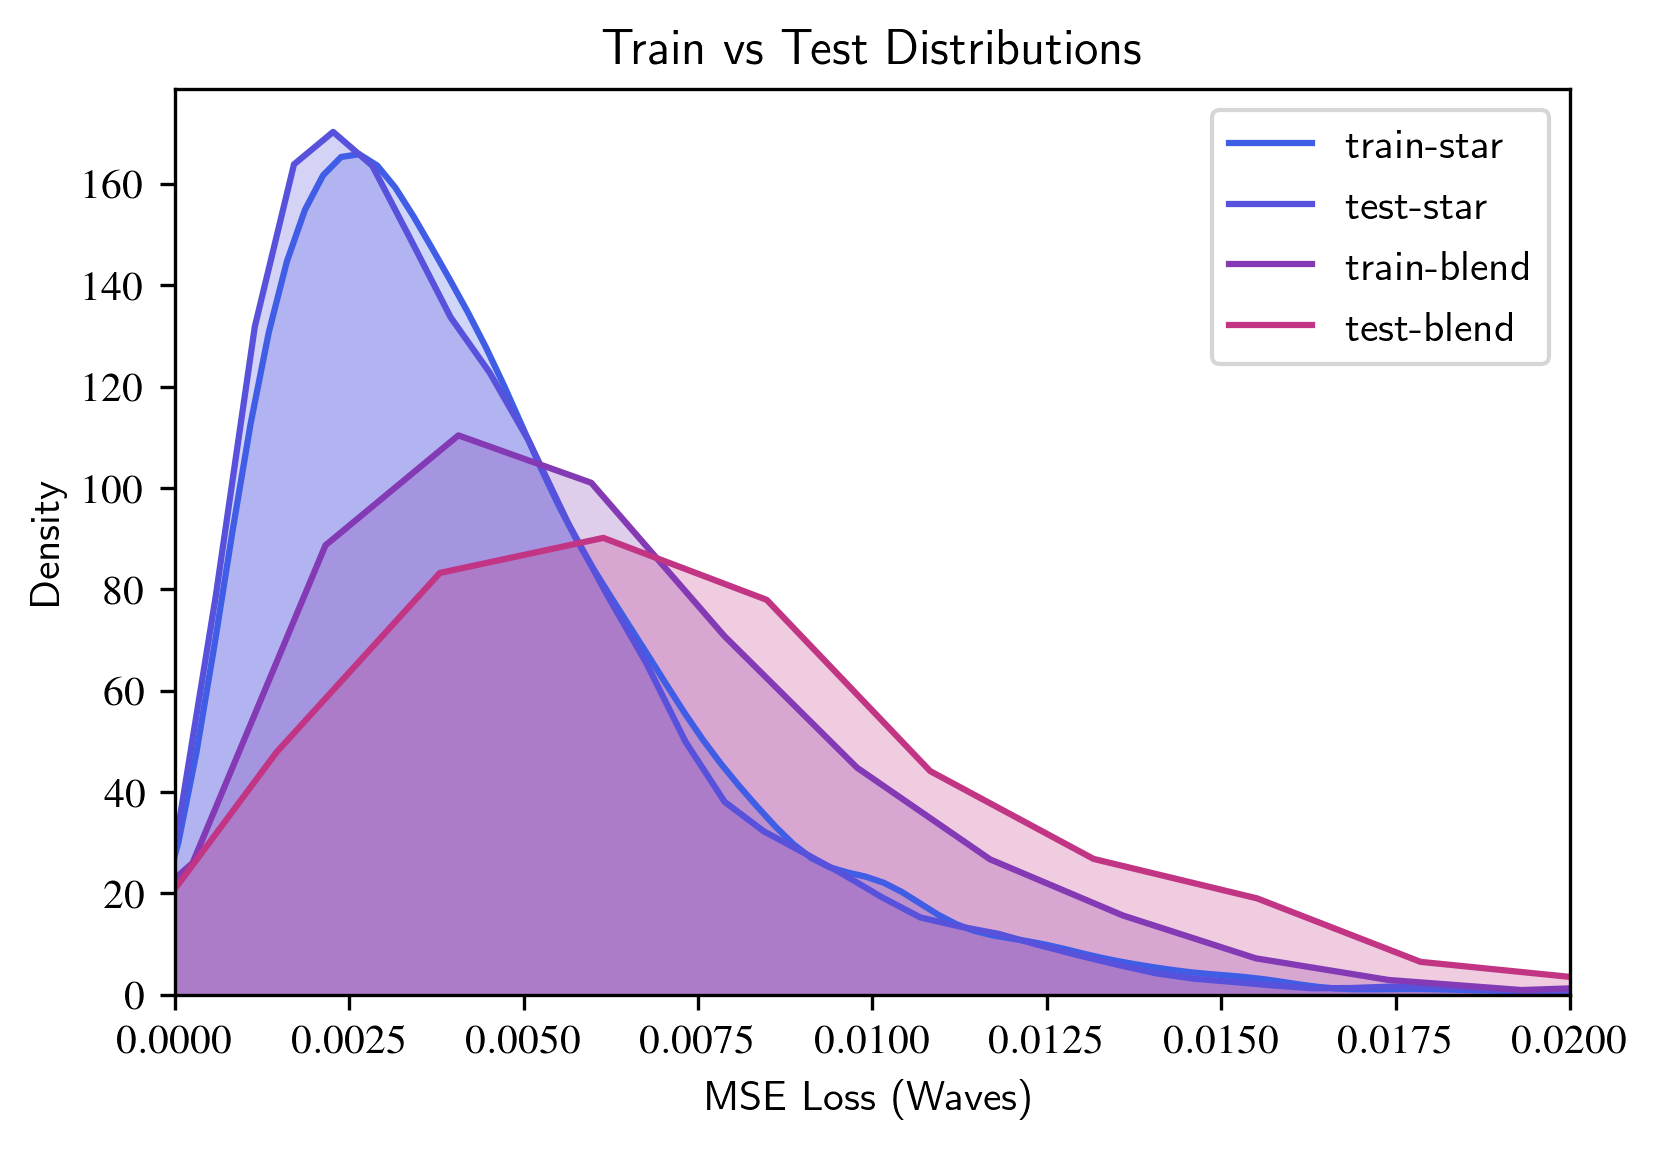
\includegraphics[width=\textwidth]{figs/cnn/train_vs_test.png}
\end{tabular}
\end{center}
\caption[Train Versus Test MSE Loss]{The distributions of the training and test MSE loss on stars (donuts with no overlaps) and blends (donuts with overlaps).\label{fig:train_vs_test}}
\end{figure}

We went through multiple iterations with different training configurations to arrive at this final configuration. To assess the models we used the validation set. Once we finalized the training configuration, we used the held out test set for a final assessment of the network. We compared the MSE loss on the training and test sets to check for overfitting. Figure \ref{fig:train_vs_test} shows the comparison. The training and test set MSE losses are $4.5\pm 3.2$ and $4.4\pm 3.5$ thousandths of waves on stars respectively, and $9.5\pm 20.0$ and $9.6\pm 22.0$ thousandths of waves on blends respectively. The performance on the training and test sets is almost identical, which suggests our model is not overfitting.

\begin{figure}[!htbp]
\begin{center}
\begin{tabular}{c}
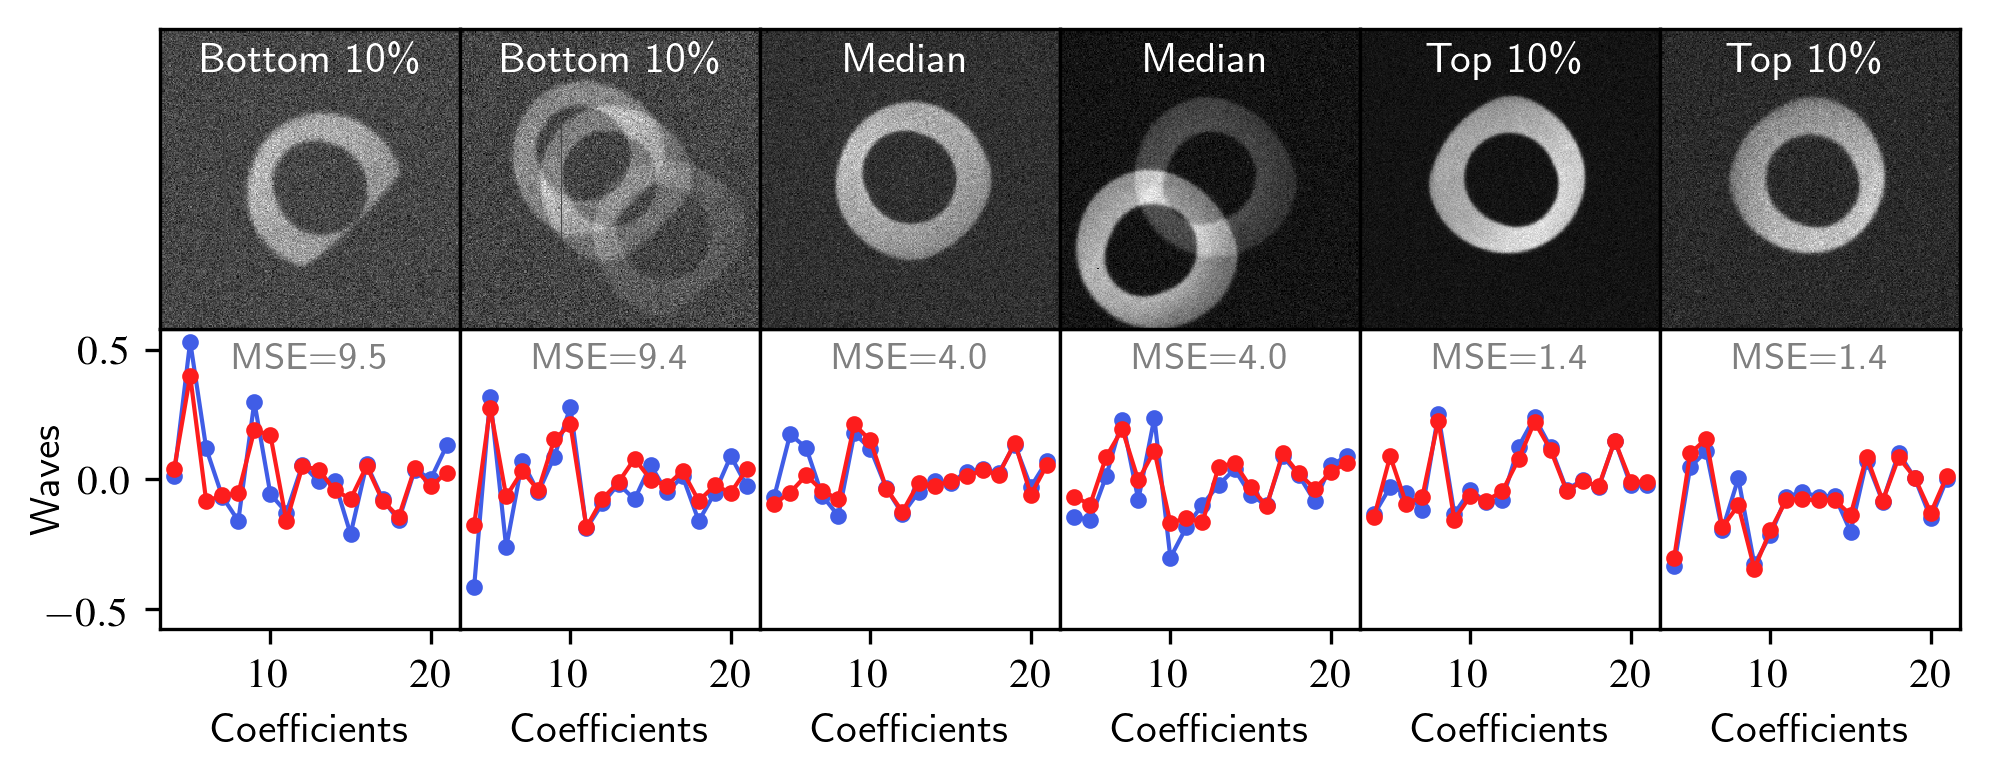
\includegraphics[width=\textwidth]{figs/cnn/donut_panel_test.png}
\end{tabular}
\end{center}
\caption[Panel of Donut Results]{Top: six donut images; two from the bottom 10\% of the MSE distribution, two from the median, and two from the top 10\%. Bottom: the corresponding true (blue) and neural network estimated (red) local wavefronts. The MSEs in the bottom row are in units of thousandths of waves.\label{fig:donut_panel}}
\end{figure}

We also inspected the performance of the network on many samples. Figure \ref{fig:donut_panel} shows the performance on six donuts from across the MSE loss distribution. At the bottom decile, the network achieves a MSE of 9.5 thousandths of a wave. While benchmarks do not exist for this task, based on our experience with other approaches and previous generation telescopes, this already seems like a competitive result. The median MSE is 4.0 thousandths of a wave. Here a few differences between the true and estimated coefficients can be seen by eye. At the top decile, the network achieves a MSE of 1.4 thousandths of a wave. The match between the true and estimated coefficients is astounding. It is perhaps more astounding to consider that the network is able to achieve this when the optics contribution that we are estimating is sub-dominant to the atmospheric contribution. 

\begin{figure}[!htbp]
\begin{center}
\begin{tabular}{c}
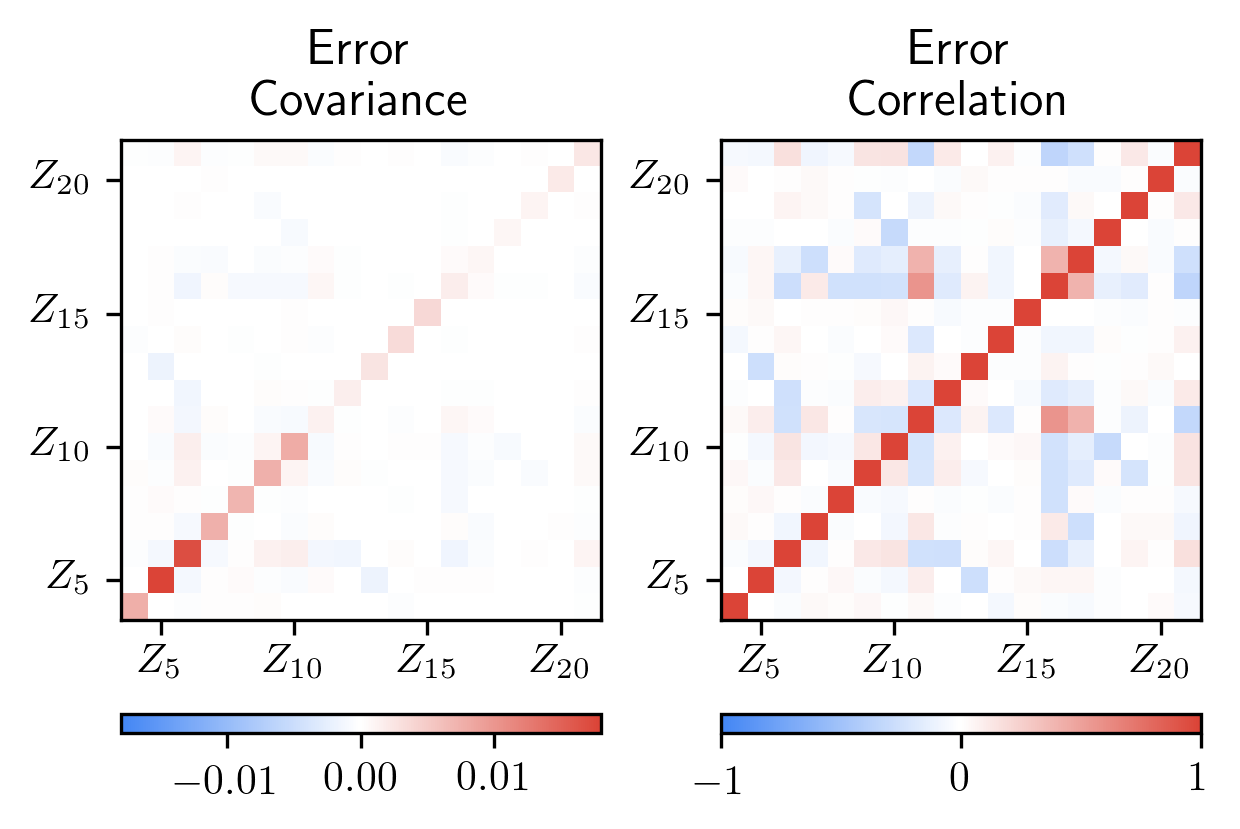
\includegraphics[width=\textwidth]{figs/cnn/cov_cor.png}
\end{tabular}
\end{center}
\caption[Wavefront Coefficient Error Covariance and Correlation]{The covariance (left) and correlation (right) of the error between different local wavefront coefficients.\label{fig:cov_cor}}
\end{figure}

It is also important to examine the correlation between the errors on different wavefront coefficients to see if there are systematic errors and biases. Figure \ref{fig:cov_cor} shows the covariance and correlation matrices for the error on the different wavefront coefficients. The covariance diagonal matches with the coefficients that are most excited in our donut dataset. For example, the $Z_5, Z_6$ astigmatism coefficients have the largest error, but also have the largest values in the true wavefront. The correlation matrix shows that the errors are fairly independent across coefficients. The largest correlations are 0.57 between $Z_{11}, Z_{16}$; 0.41 between $Z_{11},Z_{17}$; 0.40 between $Z_{16},Z_{17}$; and -0.34 between $Z_{16}, Z_{21}$.

There are a lot of parameters that determine a donut image. Another natural question is whether any of these are correlated with the error. Figure \ref{fig:err_sources} shows 8, out of the many, error sources we examined. We found that the error generally increases when the background noise increases or foreground number of photons in the donut decreases, as expected. The ratio of these contributions serves as a proxy for the signal-to-noise ratio.

Interestingly, the seeing does not have much impact, suggesting that the network is really able to differentiate between PSF contributions due to the atmosphere and due to the optics. Before training the network, we had also expected the radial distance, a proxy for the amount of vignetting, to be correlated with the error. However, in practice, it seems like the network is able to utilize the $(x,y)$ coordinates in the position to account for this effect and process vignetted donuts accurately.

\begin{figure}[!htbp]
\begin{center}
\begin{tabular}{c}
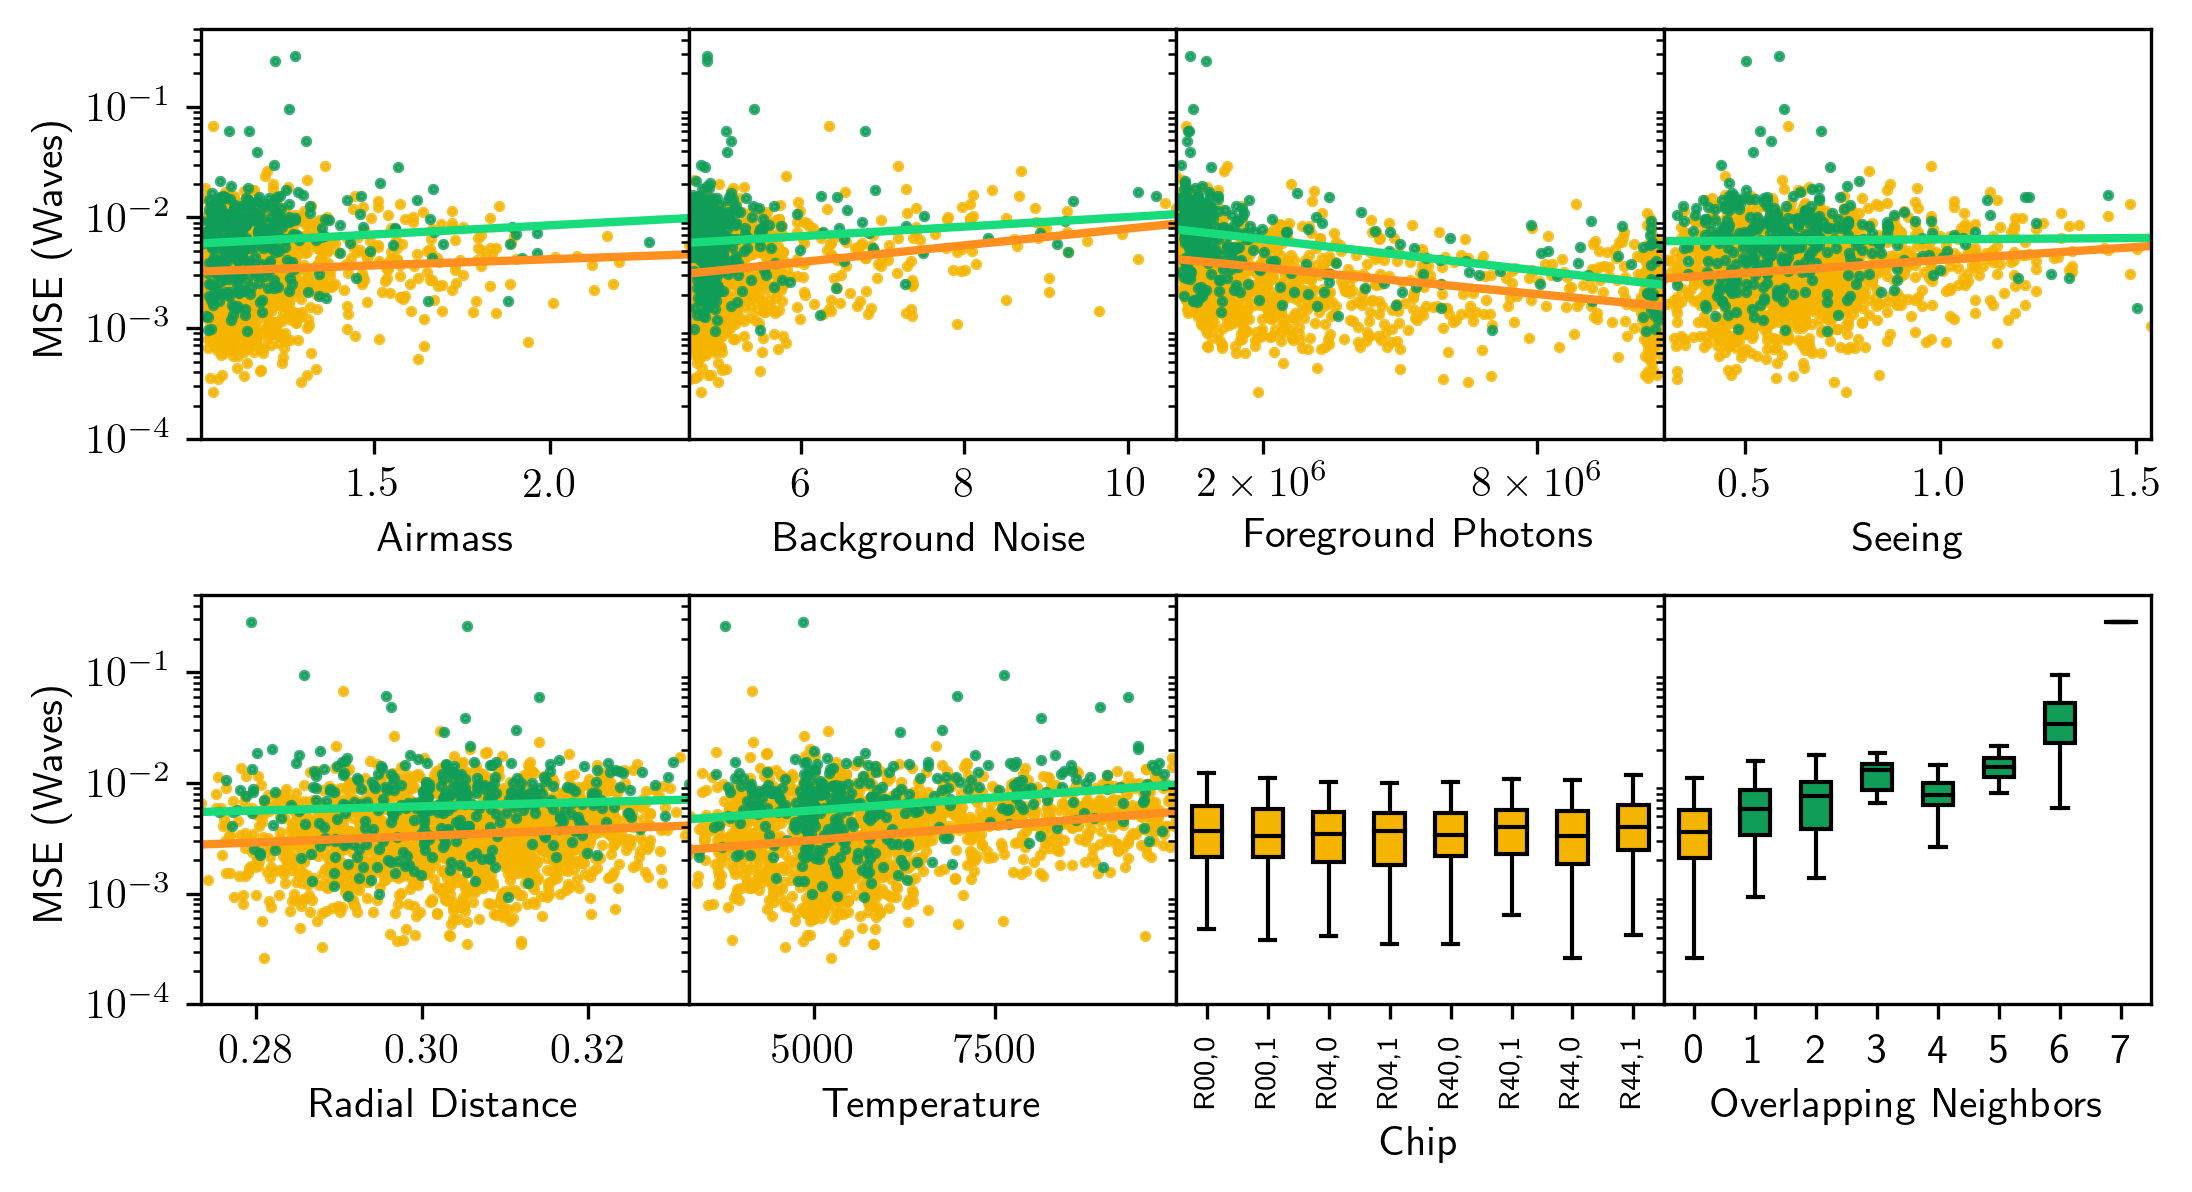
\includegraphics[width=\textwidth]{figs/cnn/error_analysis.png}
\end{tabular}
\end{center}
\caption[Panel of Potential Sources of Error]{The MSE, in waves, versus the feature distributions for 8 different potential sources of error. The stars are highlighted in yellow; the blends are in green. We also show the best fit line for the 6 non-categorical features. Units: Background Noise is the standard deviation of photons in the background, Foreground Photons is the total number of photons in the donut, Seeing is in arcseconds, Radial Distance is in meters, Temperature is in Kelvin. \label{fig:err_sources}}
\end{figure}

The biggest surprise was the impact of chromatic effects. The temperature of the source is reasonably correlated with the error. The fact that there is also some error correlation with airmass suggests some of this stems from differential chromatic refraction and some from the variations in wavelength across Rubin's r-passband and how this contributes to PSF structure. In future versions of this model, one could imagine training the network to also predict the temperature, or peak wavelength, of the source. This would better encourage it to differentiate the chromatic effects during training.

Finally, there is a clear difference between the stars (sources with no overlaps) and blends (sources with overlaps). The network performs much worse on the blends. This has important implications for which sources, and even fields, to do wavefront sensing in. As the number of overlapping neighbors increases, the error increases. However, it is important to note that there are fewer samples with large numbers of overlapping neighbors so these distributions are less reliable. In Section \ref{chap:interp}, we explore whether ignoring blends improves the performance of the global wavefront interpolation.

\section{Neural Network Enabled Insights}

At a high level, neural networks are differentiable and parameterized function approximators. The same properties that make them trainable, make them effective tools for exploring tasks in new ways. Here our network $\varphi$ has been trained to solve the task $\varphi(D, r) = \alpha$. In the next three subsections, we perform mathematical manipulations on $\varphi$ to gain insight into the behavior of our network and more general properties of this problem.

\subsection{Saliency Maps}

What aspects of the donut images is the neural network using to make its predictions? Following in the footsteps of \cite{saliency}, we define a metric that shows the pixels the predictions of the network are most sensitive to. We call this \textit{attention} and compute it by taking the magnitude of the gradient of the norm of the local wavefront prediction with respect to \textit{the pixels}. The explicit formula is

\begin{equation*}
\text{Attention}\ = \left|\nabla_D || \varphi(D, r)||_2 \right|
\end{equation*}

\noindent This gradient with respect to pixels is similar to the mechanism behind style transfer \cite{style_transfer}. 

\begin{figure}[!htbp]
\begin{center}
\begin{tabular}{c}
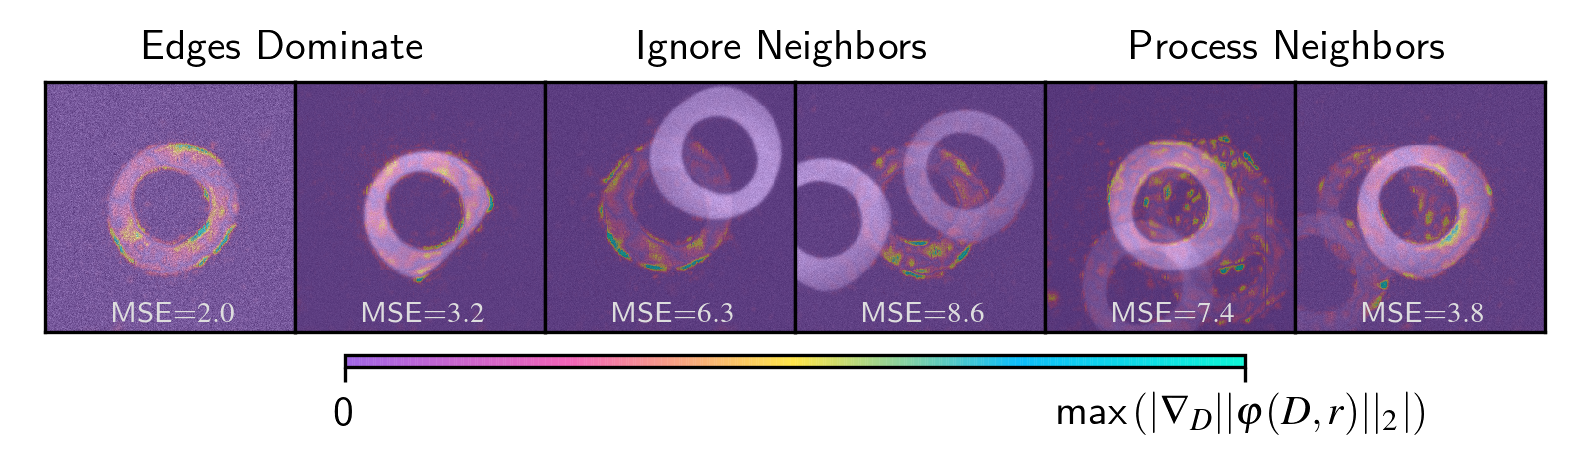
\includegraphics[width=\textwidth]{figs/cnn/attention.png}
\end{tabular}
\end{center}
\caption[Neural Network Attention]{The neural network attention values for six samples.\label{fig:attention}}
\end{figure}

Figure \ref{fig:attention} shows the attention for six samples. The first pattern that emerges is that the edges dominate, particularly when there is significant vignetting. The network focuses on the outline of a donut, in tandem with its position, to determine the wavefront. This suggests it may be possible to develop a successful network that takes only the outline of the donuts as input. It is not clear how we would have picked up this insight from the other approaches. This is an example of how the neural network can teach us new things about a problem and help us discover new approaches. 

The second pattern is that, in the case of blends, the network either utilizes or ignore the neighboring donuts. It is curious that this behavior is so bimodal. For example, where in the network is this decision being made? We suspect answering this question could unlock ways to further improve the performance of the network on blends. 

\subsection{Memorizing Versus Learning}

A common grievance of opponents to machine learning being applied in physics is that the network is memorizing, rather than truly learning, the relationships between the input and output. Here, we test this. We examine the intensity changes that would most quickly move the predictions on a base donut towards the Zernike of interest, which we deem the label-shift. We take the gradient of the norm of the difference of the network output and the target Zernike unit vector, or explicitly

\begin{equation*}
\text{Label-Shift}\ = \nabla_D || \varphi(D, r) - Z_i||_2
\end{equation*}

Figure \ref{fig:label-shift} shows the results for the Zernike unit vectors $Z_4$ through $Z_{21}$ under the respective annular Zernike polynomial. The similarity between the intensity changes and the Zernike polynomials is striking, especially given that the network has not been explicitly trained to learn these patterns. For example, the network even learns the 5 cycle periodicity of $Z_{20}$ and $Z_{21}$. It also learns the complicated radial dependence of $Z_{18}$. This demonstrates that the network is engaging in higher order learning, where it is learning general features of the problem space.

\begin{figure}[!htbp]
\begin{center}
\begin{tabular}{c}
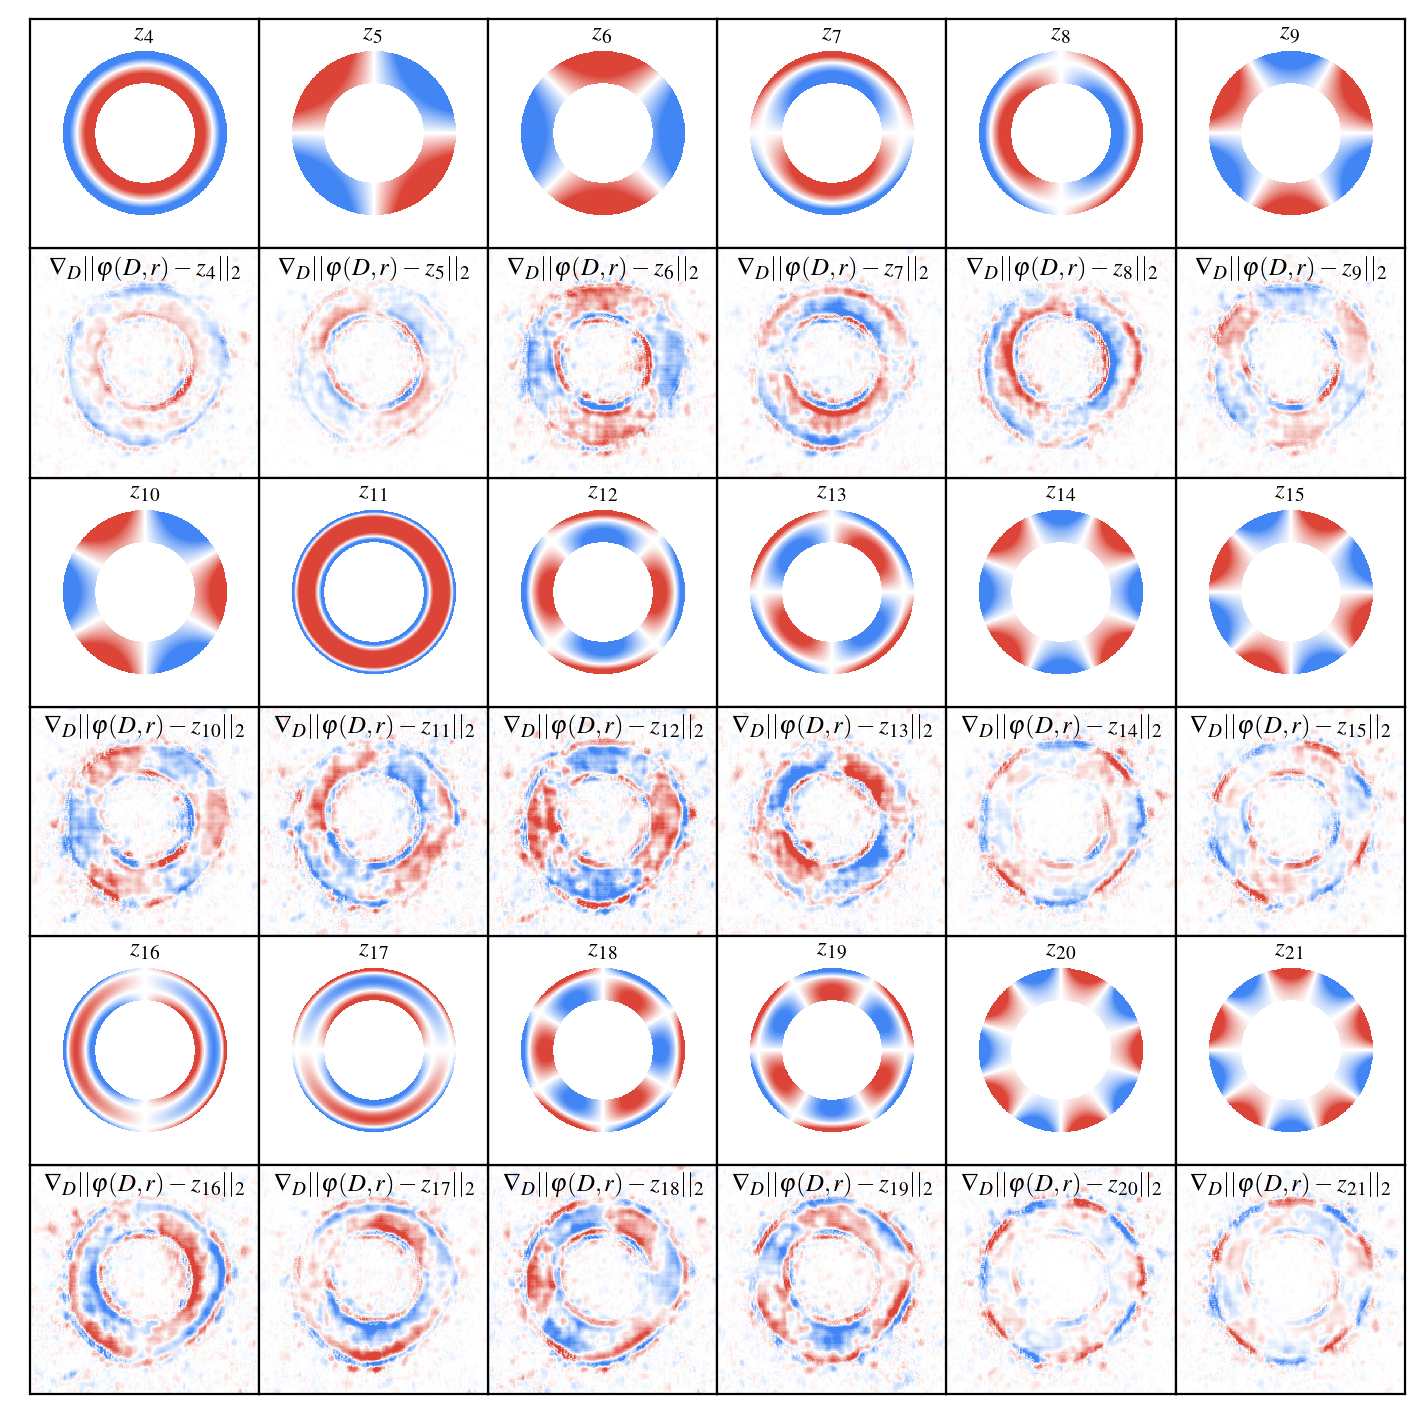
\includegraphics[width=\textwidth]{figs/cnn/morph.png}
\end{tabular}
\end{center}
\caption[Neural Network Label-Shifts]{The odd rows show the annular Zernike polynomials $Z_4$ through $Z_{21}$. The even rows show the neural network label-shifts for the corresponding Zernike unit vectors. \label{fig:label-shift}}
\end{figure}

\subsection{Adversarial Tradeoffs}

The input space for our problem, the image and the position, has $256 \times 256 + 3 = 65539$ dimensions. This is an extremely high dimensional space. It is not hard to find subtle changes in this space that are hardly discernable \textit{by eye}, or at a global level, but which can dramatically change the output of the network. In \cite{2014arXiv1412.6572G}, the authors show how to use these adversarial examples to improve training. Here, we examine a few adversarial examples to understand how our network could be hacked. 

An attacker has two competing objectives. The first is to find a modified donut image $D^\prime$ that is similar to $D$; the second is to find a modified donut image $D^\prime$ such that $\varphi(D^\prime, r)$ is close to some target $t^\prime \in \mathbb{R}^{18}$. The Adversarial-Objective is,

\begin{equation*}
\text{Adversarial-Objective}\ = ||\varphi(D^\prime, r) - t^\prime||_2^2 + ||D - D^\prime||_2^2
\end{equation*}

\noindent In order to find such a $D^\prime$ we can minimize this objective function with respect to $D^\prime$. We use the Adam optimizer to perform gradient descent. Two example results are shown in Figure \ref{fig:adversarial}. In both cases we only change one coefficient in the target $t^\prime$. 

\begin{figure}[!htbp]
\begin{center}
\begin{tabular}{c}
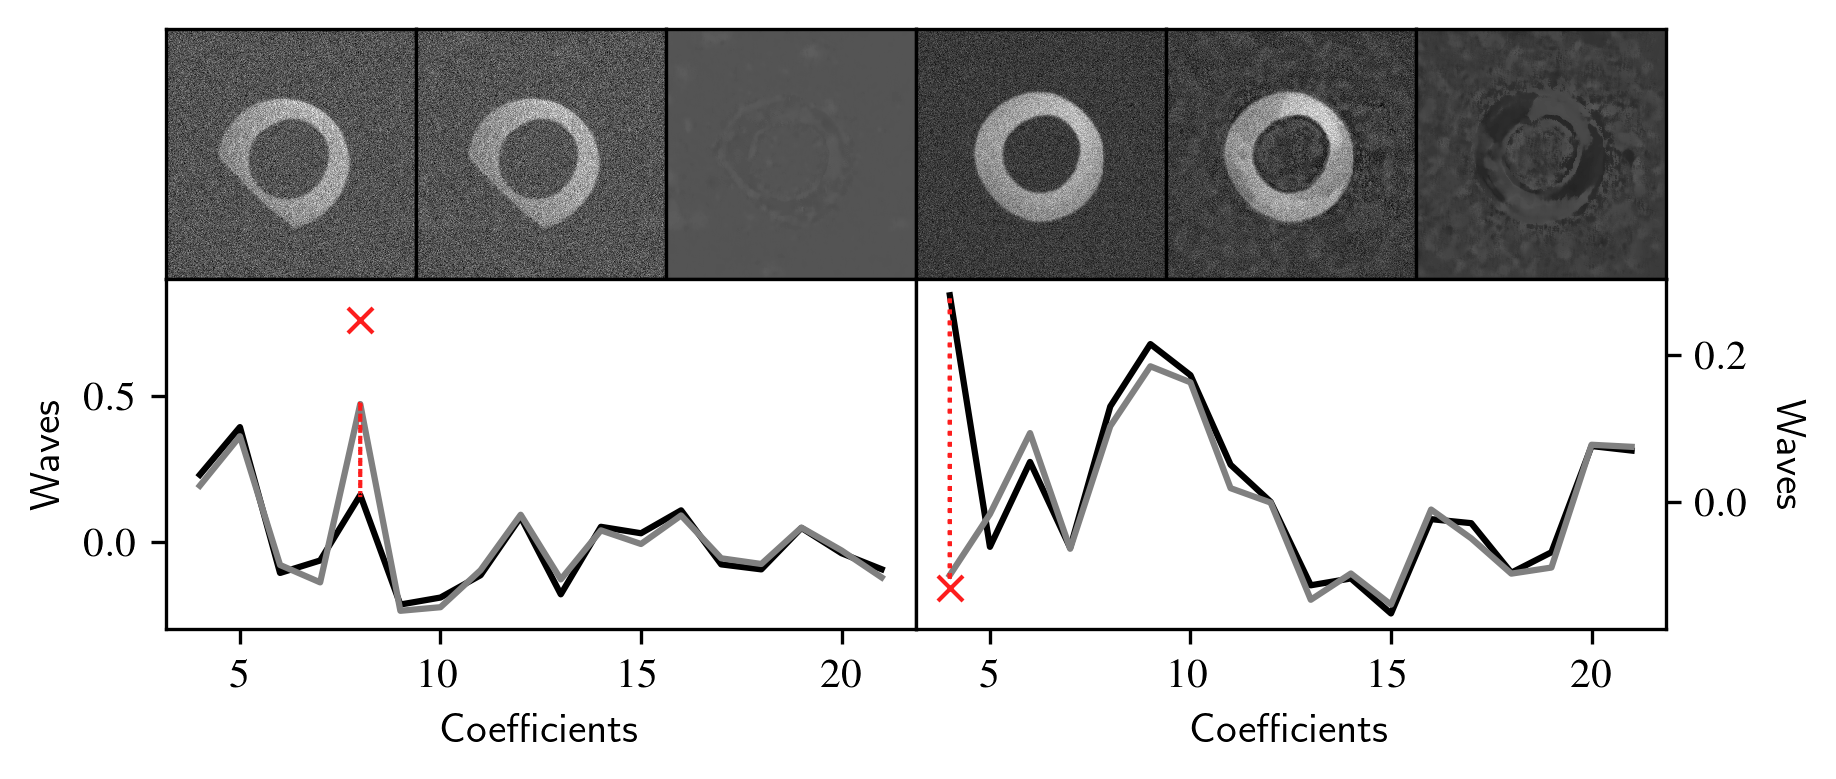
\includegraphics[width=\textwidth]{figs/cnn/adversarial.png}
\end{tabular}
\end{center}
\caption[Adversarial Attack]{Two example adversarial attacks. For each of the attacks we show three donut images, from left to right: the original donut image $D$, the new donut image $D^\prime$, and the difference $D^\prime - D$. Below we show the original prediction $\varphi(D,r)$ in black, the target $t^\prime$ as a red ``x'', and the new prediction $\varphi(D^\prime, r)$ in gray.\label{fig:adversarial}}
\end{figure}

In practice, one must scale the ratio of the two terms in the Adversarial-Objective to get good convergence. This ratio determines the relative priority of similarity between $D$ and $D^\prime$ versus $\varphi(D^\prime, r)$ and $t^\prime$. In the example on the left, we prioritized the similarity of the donuts. Here, the two donuts appear the same by eye. However, the coefficient for $Z_8$ is increased significantly, although not all the way to the target - while keeping most of the other coefficients close to their original values. This highlights the power of this kind of attack.

In the second example, the difference between the donut images is clearly discernible. Here the $Z_4$ coefficient changes dramatically, and largely hits the target, and even changes signs. This shows how the prediction can be manipulated to the target with sufficient changes to the donut. 

In the context of the Rubin Observatory, a closed environment, adverse attacks need not be feared. However, the algorithm we develop here serves a general building block for other wavefront sensing methods. These algorithms are also used for defense purposes. In this context, the sensitivity to adversarial attacks is an important characteristic to be aware of, and potentially protect against.

